
With $\kappa=12$ knobs and the standard CMA-ES population size $\lambda=11=4+\lfloor3.log(\kappa)\rfloor$, the algorithm usually lasts less than $2000\ BeATS\ evaluations$ (i.e. $180\ generations$) to converge, which is  approximately 3 hours on a regular computer without parallelization.
$U^{global}$ is set to a reasonable $5\%$, in order to give some space to CMA-ES on the global quantities.\\
The main observation, that we will develop later, is that the templates shape limit the quality of the result : in every experiment, not one but two congestion profiles appear on the contour domain and are correlated (i.e. when one grows, the other one too : they are caused by the same knob or fundamental diagram).  $\mathscr{C}$ matching the unique box $\widetilde{\mathscr{C}}$ implies that the second congestion profile is significant and outside the box.\\
We will judge the quality of the results of an experiment by the value of $J^{*}$ \emph{and} the likelyhood of the shape of the congested domain $\mathscr{C}$. \\
It is important to highlight that, for a given set of parameters, even tough the result quality is equivalent from one algorithm execution to another, the solution input $k^{*}$ found are very different. The solution of our calibration process is far from being unique for this experiment.\\
\emph{Changing the parameters:}\\
Fig. \ref{fig:results_array}. below contains the parameters and global error results of the experiments we made. We monitored the effect of each parameter by changing it slightly from one execution to another. Going in the details of each execution, we will expose in this part the effect of these parameters on the result quality. The exact values of the parameters in our case are not relevant as they depend on the scenario, time, sensor distribution, and data quality : this study is only qualitative.
\color{red}Talk on how CMA-ES always finds a way\color{black}
\begin{figure}
\centering
	\label{fig:results_array}
	\caption{Experiments parameters and $J$ final value.}
	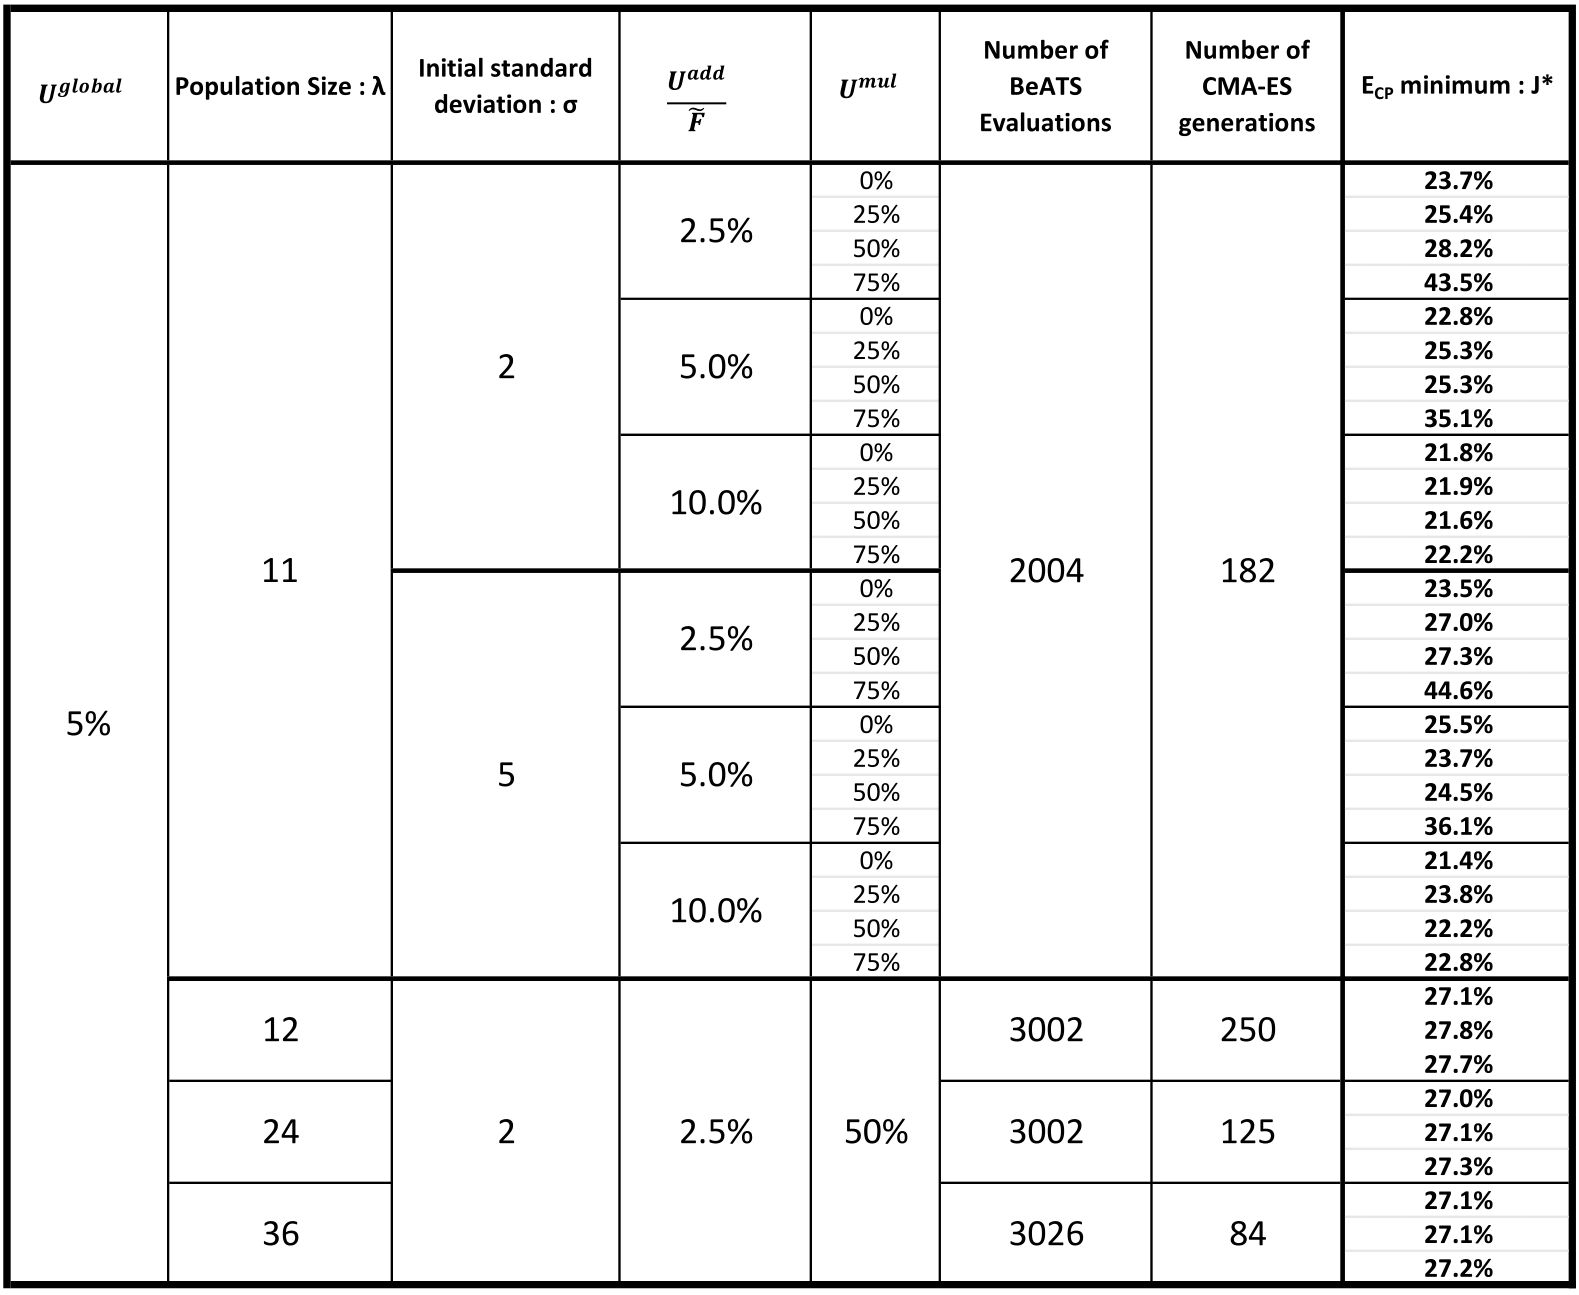
\includegraphics[width=7in]{figures/results_array.png}
\end{figure}




\begin{enumerate}
	\item Effects of changing the parameters(initial standard deviation, changing the boundaries, changing the weights, changing the uncertainty, changing size of population).
	\item Describe quality and usefulness of the result
	\item Talk about uniqueness. Way to improve (test experiment): increasing population size.\emph{Should we contact the creator of CMAES to ask him about the uniqueness of the solution (i.e. how to improve it ?}
	\item Is our problem "noisy" ?
	\item Talk about how cmaes behaves the way we want
	\item Talk about what happens when we tune also the monitored ramps knobs.	
	\item Talk about issues:
\begin{enumerate}
	\item Limit to result quality due to templates/FDS
	\item Constraints handling has to be improved because several knobs end on their boundaries values\
	\item Uncertainties are symmetric: making them fit the sensors bias (e.g. : if they always under estimate) would be better.
\end{enumerate}
	\item BLABLABLA
\end{enumerate} 
